% 2008 年陕西卷理科第 19 题：三棱锥被平行于底面 ABC 的平面所截得的几何体，
%   截面 A1B1C1，∠BAC=90°，A1A⊥平面 ABC，A1A=√3，AB=√2，AC=2，A1C1=1，BD/DC=1/2。
% 来源 PDF：gaokaomath-src/普通高考/2008/2008陕西理.pdf
% SHA-256：b6b5dd7225debdf38e60611a7b85eebe815344d38958aab6fa987ccea836dec9
% 原页：2008陕西理.pdf 第 1 页（A3 三栏）第 3 栏，书页码 475。
% 重绘依据：按原页斜投影：上底 A1（居中偏上）、B1（左）、C1（右）；下底 A（被遮挡，画在内部）、
%   B（左下）、C（右）；D 在 BC 上（BD:DC=1:2）。可见棱 A1B1、B1C1、C1A1、B1B、C1C、BC 实线；
%   被遮挡的 A1A、AB、AC 与底面中线 AD 用虚线。
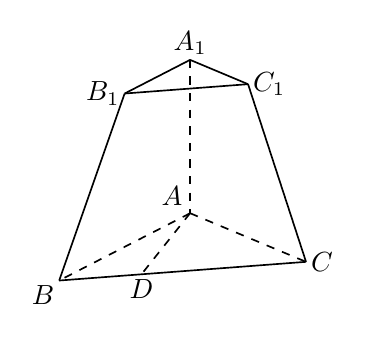
\begin{tikzpicture}[scale=0.95, semithick, every node/.style={inner sep=1.5pt}]
  \coordinate (A) at (1.05,1.00);
  \coordinate (B) at (-0.70,0.10);
  \coordinate (C) at (2.60,0.35);
  \coordinate (D) at (0.40,0.1833);
  \coordinate (A1) at (1.05,3.05);
  \coordinate (B1) at (0.175,2.60);
  \coordinate (C1) at (1.825,2.725);

  % 可见棱
  \draw (A1) -- (B1);
  \draw (B1) -- (C1);
  \draw (C1) -- (A1);
  \draw (B) -- (B1);
  \draw (C) -- (C1);
  \draw (B) -- (C);

  % 被遮挡的棱与底面中线
  \draw[dashed] (A1) -- (A);
  \draw[dashed] (A) -- (B);
  \draw[dashed] (A) -- (C);
  \draw[dashed] (A) -- (D);

  \node[above left=1pt] at (A) {$A$};
  \node[below left] at (B) {$B$};
  \node[right] at (C) {$C$};
  \node[below] at (D) {$D$};
  \node[above] at (A1) {$A_1$};
  \node[left] at (B1) {$B_1$};
  \node[right] at (C1) {$C_1$};
\end{tikzpicture}
